
\documentclass[12pt]{article}
\usepackage{graphicx,latexsym} 
\usepackage{amssymb,amsthm,amsmath}
\usepackage{longtable,booktabs,setspace} 
\usepackage{chemarr} %% Useful for one reaction arrow, useless if you're not a chem major
\usepackage[hyphens]{url}
\usepackage{rotating}
\usepackage{natbib}
\usepackage{amsthm}
\usepackage[english]{babel}
\usepackage{float}
\usepackage{graphicx}
\usepackage{amssymb}
\usepackage{hyperref}
\usepackage[utf8]{inputenc}
\usepackage{listings}
\usepackage{pgf, tikz}
\usepackage{xcolor}
\usepackage{geometry}
\usepackage [english]{babel}
\usepackage [autostyle, english = american]{csquotes}
\MakeOuterQuote{"}
\geometry{margin=1in}
\usepackage[utf8]{inputenc}
\newtheorem{theorem}{Theorem}
\newtheorem{example}{Example}
\newtheorem{remark}{Remark}[section]
\newtheorem{definition}{Definition}[section]
\newtheorem{proposition}{Proposition}[section]
\theoremstyle{definition}
\newcommand{\dsep}{\perp \!\!\!\perp}
% Comment out the natbib line above and uncomment the following two lines to use the new 
% biblatex-chicago style, for Chicago A. Also make some changes at the end where the 
% bibliography is included. 
%\usepackage{biblatex-chicago}
%\bibliography{thesis}


% Sensible defaults for lstlistings
\lstset{
  basicstyle=\footnotesize\ttfamily,
  belowcaptionskip=1\baselineskip,
  breaklines=true,
  commentstyle=\bfseries\color{purple!40!black}
  frame=L,
  identifierstyle=\color{blue},
  keywordstyle=\bfseries\color{green!40!black},
  language=python,
  showstringspaces=false,
  stringstyle=\color{orange},
}

\title{\vspace{-3cm} Recovering Joint from two Biased Distributions}
\author{Canyon Foot}


\begin{document}
\maketitle

\section{}

Here I give a simple example of two causal graphs measuring the same variables but with different selection mechanisms. In this case, the full joint distribution is recoverable only if we have access to the distributions for both graphs. We assume external information $P(x)$.


\begin{center}
\begin{tikzpicture}
  >= stealth, % arrow head style
            shorten >= 2pt, % don't touch arrow head to node
            auto,
            node distance = 3cm, % distance between nodes
            semithick % line style
        ]
        

        \tikzstyle{every state}=[
            draw = black,
            thick,
            fill = white,
            minimum size = 4mm
        ]
\node[] (X) at (2,1) {$G_1$};
\node[shape=circle,draw=black] (X) at (0,0) {X};
\node[shape=circle,draw=black] (Z) at (4,0) {Z};
\node[shape=circle,draw=black] (S) at (2,-2) {$S_1$};
\node[shape=circle,draw=black] (Y) at (0,-4) {Y};

 \path [->] (X) edge node[left] {} (Y);
  \path [->] (X) edge node[left] {} (Z);
   \path [->] (X) edge node[left] {} (S);
 \path [->] (Z) edge node[left] {} (S);
\end{tikzpicture} 
\end{center}

As always, we have access to $P(x,y,z | S_1 = 1)$, and since $Y \dsep S | X$, we also have $P(y | x)$. Additionally, since we have assumed access to $P(x)$, we could obtain $P(x,y)$ if we wanted. Notice the because of their is an edge for $Z$ to $S$, we cannot obtain $P(z)$. 

\begin{center}
\begin{tikzpicture}
  >= stealth, % arrow head style
            shorten >= 2pt, % don't touch arrow head to node
            auto,
            node distance = 3cm, % distance between nodes
            semithick % line style
        ]
        

        \tikzstyle{every state}=[
            draw = black,
            thick,
            fill = white,
            minimum size = 4mm
        ]
\node[] (X) at (2,1) {$G_2$};
\node[shape=circle,draw=black] (X) at (0,0) {X};
\node[shape=circle,draw=black] (Z) at (4,0) {Z};
\node[shape=circle,draw=black] (S) at (2,-2) {$S_2$};
\node[shape=circle,draw=black] (Y) at (0,-4) {Y};

 \path [->] (X) edge node[left] {} (Y);
  \path [->] (X) edge node[left] {} (Z);
   \path [->] (X) edge node[left] {} (S);
 \path [->] (Y) edge node[left] {} (S);
\end{tikzpicture} 
\end{center}

The story here is similar. We can get $P(x,y,z | S_2 = 1)$,  $P(z | x)$, and $P(x,z)$ (using the external data). Then, using the chain rule for probability,

\begin{align*}
P(X,Y,Z) &= P(Y | X, Z) P(X,Z) \\
&= P(Y | X) P(Z | X) P(X) 
\end{align*}

Since we have all of these quantities we can find $P(X,Y,Z)$ without issue. However, to do so we need to use $P(Z | X)$ and $P(Y | X)$, which means we need both biased distributions. To really investigate what happens when multiple selection biased distributions are present, we will want to express the selection mechanisms within a single graph. To do so, we simply 'superimpose' the graphs. So, for our current example, we get a new graph:

\begin{center}
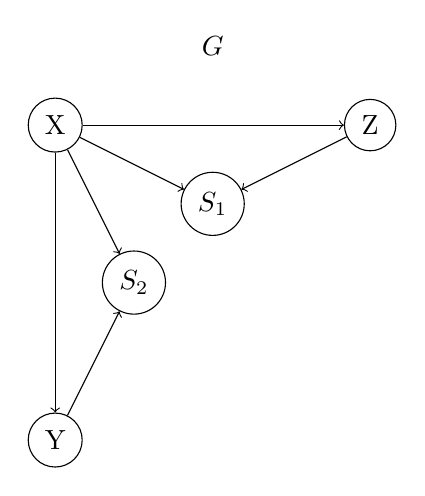
\begin{tikzpicture}
  >= stealth, % arrow head style
            shorten >= 2pt, % don't touch arrow head to node
            auto,
            node distance = 3cm, % distance between nodes
            semithick % line style
        ]
        

        \tikzstyle{every state}=[
            draw = black,
            thick,
            fill = white,
            minimum size = 4mm
        ]
\node[] (X) at (2,1) {$G$};
\node[shape=circle,draw=black] (X) at (0,0) {X};
\node[shape=circle,draw=black] (Z) at (4,0) {Z};
\node[shape=circle,draw=black] (S1) at (2,-1) {$S_1$};
\node[shape=circle,draw=black] (S2) at (1, -2) {$S_2$};
\node[shape=circle,draw=black] (Y) at (0,-4) {Y};

 \path [->] (X) edge node[left] {} (Y);
  \path [->] (X) edge node[left] {} (Z);
   \path [->] (X) edge node[left] {} (S2);
 \path [->] (Y) edge node[left] {} (S2);
  \path [->] (X) edge node[left] {} (S1);
    \path [->] (Z) edge node[left] {} (S1);
\end{tikzpicture} 
\end{center}

A few things of note. We do not allow the selection nodes $S_1$ and $S_2$ to have children, and therefore any path passing through a selection node (i.e. $V \rightarrow S_i \leftarrow W$) will include a collider at $S_1$. This means that the definition of path blocking gives that any such path is blocked, and therefore any d-separation statement that holds in one of the original graphs will hold in the superimposed graph. This fact allows us to apply the first and second theorems from Barenboim 2014 to get the following propositions.

\begin{proposition}
A conditional distribution $P(y | \mathbf{x})$ can be recovered from a if there is a selection node $S_i$ such that $Y \dsep S_i | \mathbf{X} $.
\end{proposition}
And similarly,

\begin{proposition}
When external information $P(\mathbf{x}, \mathbf{c})$ is available, the conditional distribution $P(y | x)$ is recoverable if there is a selection node $S_i$ such that $Y \dsep S_i | (\mathbf{X}, \mathbf{C})$.
\end{proposition} 
 
These propositions are little more than sanity checks since they state that any distribution recoverable from one of the biased distribution alone is recoverable when all are accessible. What is more interesting is establishing the criteria under which distributions not recoverable from any of the biased distributions in isolation are recoverable when the collection of distributions are accessible. 
\end{document}
 